\section{Matplotlib}

\subsection{figureとaxes}
一つ一つのグラフの本体は,Matplotlibでは\texttt{axes}オブジェクトとして表され,\texttt{axes}オブジェクトは,\texttt{figure}オブジェクトの中で管理される.イメージとしては、\texttt{figure}オブジェクトは白のキャンバスであり,そこにグラフの素である\texttt{axes}オブジェクトを置いていく.

\begin{cod}[\texttt{fig1.py}] 
\lstinputlisting[backgroundcolor={\color[gray]{.95}}]{code/fig1.py}
\vspace{-15pt}
\begin{figure}[H]
\begin{center}
\framed
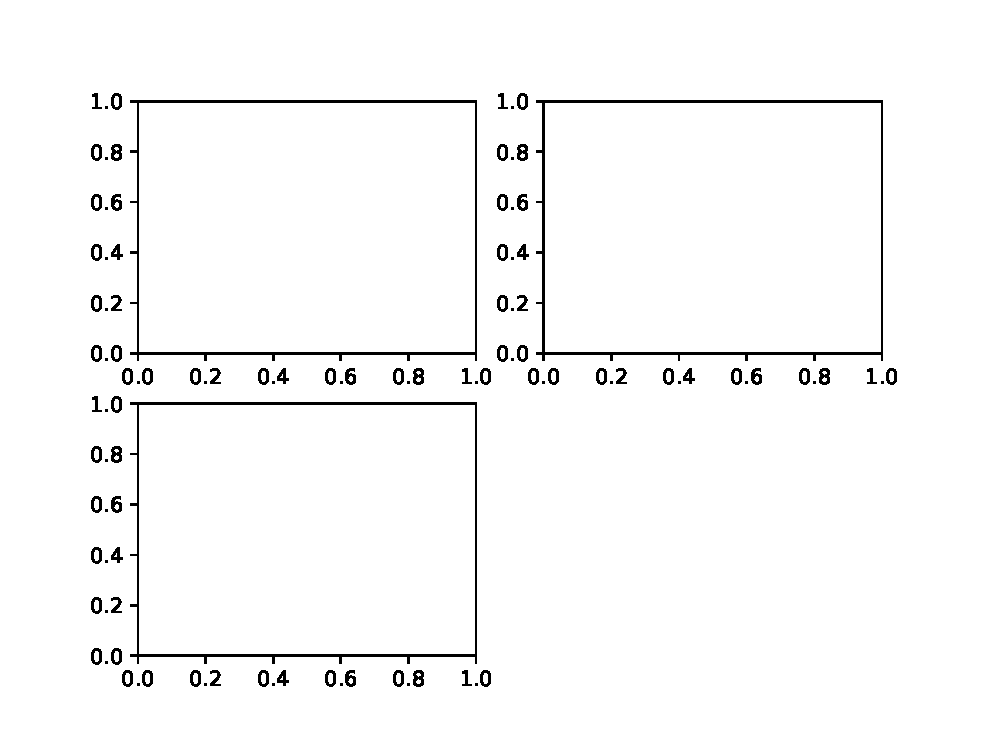
\includegraphics[width=10.0cm]{code/fig1.eps}
\endframed
\end{center}
\end{figure}
%\begin{lstlisting}
%\end{lstlisting}
\end{cod}
\vspace{-20pt}
\begin{itemize}
\item \texttt{plt.figure()}: 空の\texttt{figure}オブジェクトを作成する.
\item \texttt{[figure].add\_subplot(a,b,c)}: \texttt{figure}オブジェクトを$a$行$b$列に分割した上で,$c$番目の部分に空の\texttt{axes}オブジェクトを作成する.
\item \texttt{[figure].savefig('XXXX.XXX')}: ~\texttt{figure}オブジェクトを\texttt{XXXX.XXX}として保存する.
\end{itemize}

\subsection{散布図}

まずはじめに散布図を描画してみよう.
\begin{cod}[\texttt{fig2.py}] 
\lstinputlisting[backgroundcolor={\color[gray]{.95}}]{code/fig2.py}
\vspace{-15pt}
\begin{figure}[H]
\begin{center}
\framed
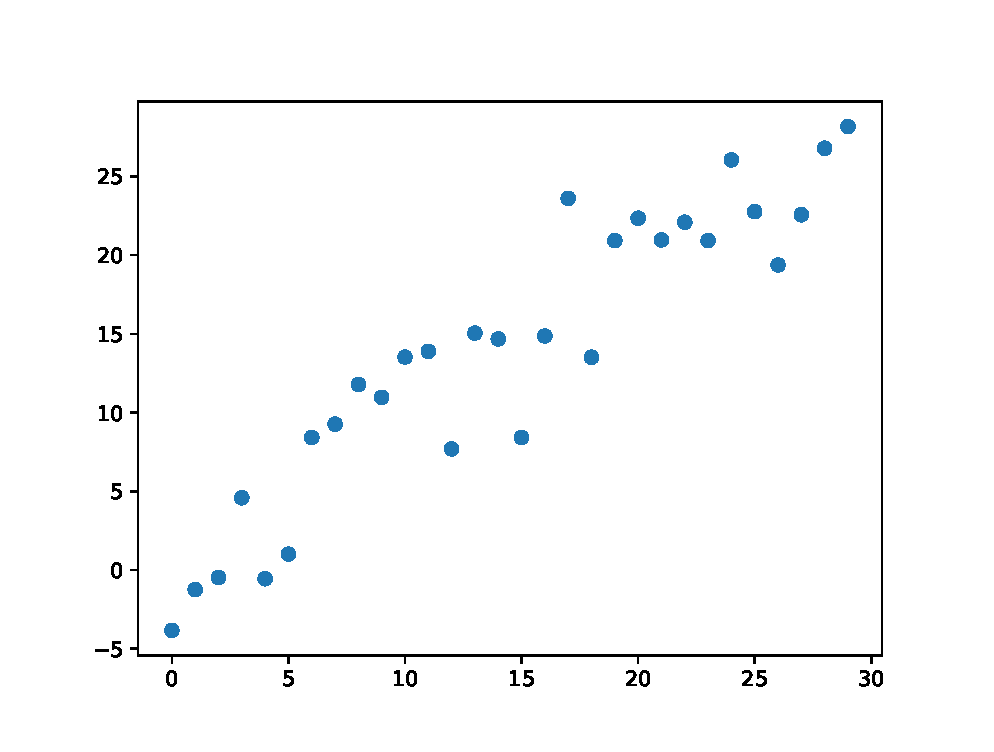
\includegraphics[width=8.0cm]{code/fig2.eps}
\endframed
\end{center}
\end{figure}
%\begin{lstlisting}
%\end{lstlisting}
\end{cod}
\vspace{-20pt}